% =============================================================================
% TEMPLATE DE ARTIGO - PROJETO DE PESQUISA EM COMPUTAÇÃO GRÁFICA
% Bacharelado em Ciência da Computação - IFNMG - Campus Montes Claros
% Disciplina: Computação Gráfica - 2026/2
% Professor: Wagner Ferreira de Barros
%
% Formato didático inspirado em características recorrentes de conferências de
% Computação Gráfica (p.ex., ACM SIGGRAPH/SIGGRAPH Asia e Eurographics):
% texto compacto, duas colunas, corpo em 9 pt, pequeno espaçamento vertical e
% figuras/tabelas integradas ao fluxo.
%
% IMPORTANTE: este é o modelo oficial DA DISCIPLINA, não o template oficial de
% um evento específico. Para futura submissão, migre o conteúdo para o template
% oficial do evento escolhido e siga integralmente as regras daquela chamada.
%
% Extensão exigida na disciplina: 8 a 12 páginas, incluindo referências.
% =============================================================================

\documentclass[9pt,a4paper,twocolumn]{extarticle}

% -----------------------------------------------------------------------------
% Codificação, idioma e tipografia
% -----------------------------------------------------------------------------
\usepackage[T1]{fontenc}
\usepackage[utf8]{inputenc}
\usepackage[brazil]{babel}
\usepackage{newtxtext,newtxmath}
\usepackage{microtype}

% -----------------------------------------------------------------------------
% Página e colunas
% Área útil próxima aos padrões compactos usados em publicações de CG.
% -----------------------------------------------------------------------------
\usepackage[a4paper,textwidth=177mm,textheight=245mm,centering]{geometry}
\setlength{\columnsep}{8mm}
\setlength{\columnseprule}{0pt}
\setlength{\parindent}{1em}
\setlength{\parskip}{0pt}
\linespread{0.97}
\pagestyle{empty}

% -----------------------------------------------------------------------------
% Seções compactas
% -----------------------------------------------------------------------------
\usepackage{titlesec}
\titleformat{\section}
  {\normalfont\bfseries\fontsize{10.5}{11.5}\selectfont}
  {\thesection}{0.5em}{}
\titleformat{\subsection}
  {\normalfont\bfseries\fontsize{9.5}{10.5}\selectfont}
  {\thesubsection}{0.45em}{}
\titlespacing*{\section}{0pt}{7pt plus 2pt minus 1pt}{3pt}
\titlespacing*{\subsection}{0pt}{5pt plus 1pt minus 1pt}{2pt}

% -----------------------------------------------------------------------------
% Figuras, tabelas, matemática e listas
% -----------------------------------------------------------------------------
\usepackage{graphicx}
\graphicspath{{./figures/}}
\usepackage{booktabs}
\usepackage{tabularx}
\usepackage{array}
\usepackage{amsmath}
\usepackage{siunitx}
\usepackage{subcaption}
\usepackage{balance}
\usepackage{enumitem}
\setlist[itemize]{leftmargin=1.25em,itemsep=0pt,topsep=2pt,parsep=0pt}
\setlist[enumerate]{leftmargin=1.5em,itemsep=0pt,topsep=2pt,parsep=0pt}

% -----------------------------------------------------------------------------
% Legendas compactas
% -----------------------------------------------------------------------------
\usepackage[font=small,labelfont=bf]{caption}
\captionsetup{skip=3pt}
\setlength{\textfloatsep}{7pt plus 2pt minus 2pt}
\setlength{\floatsep}{6pt plus 2pt minus 2pt}
\setlength{\intextsep}{6pt plus 2pt minus 2pt}

% -----------------------------------------------------------------------------
% Referências e links
% -----------------------------------------------------------------------------
\usepackage[backend=biber,style=authoryear,maxcitenames=2,maxbibnames=20]{biblatex}
\addbibresource{referencias.bib}
\usepackage[hidelinks]{hyperref}
\usepackage{url}

% -----------------------------------------------------------------------------
% Código-fonte
% -----------------------------------------------------------------------------
\usepackage{xcolor}
\usepackage{listings}
\definecolor{codegray}{gray}{0.45}
\definecolor{codegreen}{rgb}{0.0,0.40,0.0}
\definecolor{codeblue}{rgb}{0.10,0.20,0.65}
\lstset{
  basicstyle=\ttfamily\scriptsize,
  keywordstyle=\color{codeblue}\bfseries,
  commentstyle=\color{codegreen},
  numberstyle=\tiny\color{codegray},
  numbers=left,
  numbersep=4pt,
  frame=single,
  aboveskip=4pt,
  belowskip=4pt,
  breaklines=true,
  showstringspaces=false,
  columns=fullflexible
}

% -----------------------------------------------------------------------------
% Orientações didáticas
% Troque para \mostrarorientacoesfalse antes da entrega final.
% -----------------------------------------------------------------------------
\newif\ifmostrarorientacoes
\mostrarorientacoestrue

\newcommand{\orientacao}[1]{%
  \ifmostrarorientacoes
    \par\smallskip
    \noindent\fcolorbox{black!35}{black!4}{%
      \parbox{0.94\columnwidth}{\fontsize{7.4}{8.2}\selectfont\textbf{Orientação aos autores:} #1}%
    }%
    \par\smallskip
  \fi
}

% =============================================================================
% DOCUMENTO
% =============================================================================
\begin{document}

% Título e resumo em largura total, seguido do corpo em duas colunas.
\twocolumn[
\begin{center}
  {\sffamily\bfseries\fontsize{14}{16}\selectfont
   Modelagem e Simulação Procedural de Rios Meândricos com Modulação Espacial por Mobilidade Litológica Relativa\par}
  \vspace{5pt}
  {\fontsize{9.5}{11}\selectfont
   Alberto Henrique \quad Pedro Henrique Braga \quad Warley Ramires\par}
  \vspace{2pt}
  {\fontsize{8.5}{10}\selectfont
   Orientador: Prof. Dr. Wagner Ferreira de Barros\par
   Instituto Federal do Norte de Minas Gerais -- IFNMG, Campus Montes Claros\par
   \texttt{warleyramiresgoncalves@gmail.com}\par}
\end{center}
\vspace{3pt}

\begin{minipage}{0.94\textwidth}
\fontsize{8.5}{9.5}\selectfont
\noindent\textbf{Resumo.}
A síntese procedural de redes hidrográficas e planícies aluviais é um problema central na modelagem de terrenos virtuais em Computação Gráfica. Métodos recentes baseados em curvas paramétricas simulam com alta eficiência a migração lateral, o estrangulamento de meandros (\textit{cutoffs}) e eventos de avulsão em escala de quilômetros, mas assumem erodibilidade lateral uniforme ao longo do substrato. Neste trabalho, investigamos e implementamos uma extensão geomorfológica leve que introduz um campo escalar bidimensional independente de mobilidade litológica relativa $E(x,y)$, amostrado na margem externa (\textit{cut bank}) do canal fluvial a uma distância de meia largura da linha central. O fator de mobilidade normalizado $g(E) = \text{clamp}(E/\bar{E}, g_{\min}, g_{\max})$ modula multiplicativamente a taxa cinemática de migração. A implementação foi validada por regressão numérica sob substrato homogêneo ($L_\infty \le 10^{-9}$ em relação à baseline) e avaliada quanto ao impacto de heterogeneidades litológicas na trajetória e estabilidade numérica do canal.

\vspace{3pt}
\noindent\textbf{Palavras-chave:} Computação Gráfica; Modelagem Procedural de Terrenos; Rios Meândricos; Mobilidade Litológica.

\vspace{5pt}
\noindent\textbf{Abstract.}
Procedural synthesis of river networks and alluvial plains is a core problem in virtual terrain modeling in Computer Graphics. Recent parametric curve-based methods efficiently simulate lateral migration, neck cutoffs, and avulsion events at kilometer scales, yet assume uniform lateral erodibility across the substrate. In this work, we investigate and implement a lightweight geomorphological extension that introduces an independent 2D scalar field of relative lithologic mobility $E(x,y)$, sampled at the external bank (cut bank) of the river channel at half-width distance from the centerline. The normalized mobility factor $g(E) = \text{clamp}(E/\bar{E}, g_{\min}, g_{\max})$ multiplicatively modulates the kinematic migration rate. We validate our implementation through numerical regression under homogeneous substrates ($L_\infty \le 10^{-9}$ against the baseline) and evaluate the impact of lithologic heterogeneity on channel trajectory and numerical stability.

\vspace{3pt}
\noindent\textbf{Keywords:} Computer Graphics; Procedural Terrain Modeling; Meandering Rivers; Lithologic Mobility.
\end{minipage}
\vspace{8pt}
]

% =============================================================================
\section{Introdução}
% =============================================================================
\orientacao{Contextualize o problema de Computação Gráfica, explique sua relevância,
apresente o trabalho de referência e conduza o leitor até a questão específica investigada.
A introdução deve terminar com a questão/hipótese e as contribuições do artigo.}

A geração realista de terrenos virtuais é um requisito essencial em jogos eletrônicos, simuladores de treinamento, cinema e visualização científica. Enquanto técnicas clássicas baseadas em ruído coerente (como Perlin ou Simplex) produzem relevos montanhosos plausíveis a baixo custo, elas falham em capturar a estrutura espacial e a evolução temporal de sistemas fluviais em planícies aluviais dominadas por rios meândricos. No extremo oposto, simulações físicas baseadas em dinâmica dos fluidos computacional (CFD) tridimensional apresentam custo computacional proibitivo para domínios extensos e fluxos de autoria interativa.

Para conciliar realismo geomorfológico, controle artístico e baixo tempo de execução, \textcite{paris2023meandering} propuseram um arcabouço cinemático-geométrico para autoria e simulação de rios meândricos. Apesar de considerar a atenuação da migração pela declividade topográfica ($\nabla h$) e por restrições autorais, o método original assume que o substrato geológico possui erodibilidade lateral uniforme em todo o domínio. Na natureza, contudo, planícies fluviais interceptam unidades litológicas distintas --- como barreiras rochosas resistentes ou lentes de sedimentos friáveis --- que restringem ou aceleram localmente a erosão da margem externa (\textit{cut bank}).

Este trabalho investiga a seguinte questão de pesquisa: \textit{``Como a introdução de uma matriz bidimensional de mobilidade litológica relativa $E(x,y)$, independente da topografia e amostrada na margem externa do canal, modula a taxa de migração lateral, a morfometria (sinuosidade e comprimento de onda) e a estabilidade numérica de rios meândricos procedurais?''}. As contribuições deste artigo incluem: (i) reprodução e isolamento da baseline pública de \textcite{paris2023meandering}; (ii) formulação e implementação de um operador de amostragem litológica na margem externa normalizado pela média espacial $\bar{E}$; e (iii) validação por testes de regressão e experimentos controlados de ablação.

% =============================================================================
\section{Trabalho de Referência e Trabalhos Relacionados}
% =============================================================================
\orientacao{Apresente o artigo-base com precisão suficiente para que o leitor entenda
a técnica que será modificada. Discuta apenas a literatura necessária para posicionar
a proposta. Verifique trabalhos posteriores antes de afirmar novidade.}

Na Computação Gráfica, os primeiros métodos de geração de redes hidrográficas integraram canais de baixa resolução diretamente à síntese do relevo por deslocamento de ponto médio \parencite{kelley1988terrain} e regras de subdivisão estocástica \parencite{prusinkiewicz1993fractal}. Abordagens posteriores passaram a construir árvores fluviais hidrologicamente consistentes com a classificação geomorfológica de Rosgen, escavando o leito a partir de curvas de controle e perfis pré-definidos \parencite{genevaux2013terrain, peytavie2019procedural}. Como esses algoritmos tratam os rios como estruturas geométricas estáticas, o traçado gerado não evolui no tempo e omite feições típicas de planícies aluviais, a exemplo de meandros abandonados. Em outra vertente, simulações hidráulicas baseadas em partículas \parencite{kristof2009hydraulic} ou equações de águas rasas \parencite{benes2006hydraulic} reproduzem o transporte de sedimentos em pequena escala, porém exigem alto tempo de processamento e oferecem pouco controle direto sobre a trajetória dos canais. Modelos de erosão fluvial em escala tectônica baseados na lei da potência do fluxo (\textit{stream power}) \parencite{cordonnier2016large, schott2023large} geram bacias de drenagem extensas e coerentes, mas operam em resoluções espaciais e temporais que impedem a formação da dinâmica lateral de rios meândricos.

Nas Geociências, a evolução temporal de canais meândricos é tradicionalmente modelada representando o rio por sua linha central discretizada. Os trabalhos clássicos de \textcite{ikeda1981bend} e \textcite{howard1984sufficient} estabeleceram que a velocidade de erosão da margem depende da curvatura local combinada com a influência acumulada das curvaturas a montante. A partir de medições de alta precisão em rios reais, \textcite{sylvester2019high} confirmaram essa relação linear e demonstraram que a ponderação das curvaturas anteriores introduz um atraso espacial (\textit{lag}) entre o ponto de curvatura máxima e o ponto de migração máxima, deslocando as alças meândricas progressivamente para jusante. Embora simuladores estratigráficos baseados em processos, como o modelo de \textcite{lopez2009process}, incorporem variações de fácies e tipos de rocha para reconstruir reservatórios tridimensionais ao longo de eras geológicas, esses sistemas tratam apenas canais isolados sem interação com a topografia circundante nem ferramentas de edição em tempo real.

Tomando como base a formulação de \textcite{sylvester2019high}, o trabalho de referência de \textcite{paris2023meandering} estende a simulação de linha central para redes fluviais completas em terrenos de múltiplos quilômetros. Cada canal é representado no plano por uma curva spline cúbica por partes composta por vértices ordenados $\mathbf{p}_i \in \mathbb{R}^2$, largura constante $w$ e profundidade $d$. A taxa de migração local em cada ponto é dada por $R_0(i) = k_1 w C(i)$, onde $k_1$ é a constante de velocidade de migração e $C(i)$ é a curvatura discreta calculada por diferenças centrais. Para incorporar o efeito da geometria a montante ao longo da distância curvilinear $s_{i, i-k}$, o método calcula a taxa efetiva $\mu_{\text{base}}(i)$ usando um núcleo de decaimento exponencial $G(k) = \exp(-\alpha s_{i,i-k})$, com $\alpha = 2 k C_f / d$ definido pelo fator de atrito $C_f$ e pela profundidade do canal:
\begin{equation}
    \mu_{\text{base}}(i) = \sigma^{-2/3} \left( \Omega R_0(i) + \Gamma \frac{\sum_{k \ge 0} R_0(i-k) \, G(k)}{\sum_{k \ge 0} G(k)} \right),
    \label{eq:total_migration}
\end{equation}
em que $\sigma$ é a sinuosidade do canal, $\Omega = -1{,}0$ e $\Gamma = 2{,}5$. Como o deslocamento lateral altera o espaçamento entre vértices adjacentes, a curva é reconstruída e reamostrada a intervalos regulares $\Delta s \le w$ ao final de cada passo de tempo $\Delta t$.

Para acoplar a simulação geomorfológica ao relevo e à edição interativa, \textcite{paris2023meandering} ponderam o deslocamento de cada ponto pela equação:
\begin{equation}
    \mathbf{p}_i(t + \Delta t) = \mathbf{p}_i(t) + w_f(i) \, w_t(i) \, \Delta t \, \mu_{\text{base}}(i) \, \mathbf{d}_{\text{mig}}(i).
    \label{eq:baseline_step}
\end{equation}
O termo $w_f(i) \in [0, 1]$ reduz a migração próximo às extremidades do canal para preservar a posição estática das junções da rede, enquanto $w_t(i) \in [0, 1]$ aplica uma função de transição suave sobre a declividade local $\|\nabla h(\mathbf{p}_i)\|^2$, anulando o meandramento em encostas íngremes e mantendo trajetórias retilíneas em zonas montanhosas. O vetor $\mathbf{d}_{\text{mig}}(i)$ combina a normal unitária do canal com o gradiente de regiões atrativas ou repulsivas definidas pelo usuário. Além da migração contínua, o método resolve eventos abruptos a cada passo: quando dois pontos não consecutivos se aproximam a uma distância inferior à largura $w$, um operador de estrangulamento (\textit{cutoff}) reconecta o segmento mais curto e armazena a alça abandonada como um lago em ferradura (\textit{oxbow lake}); em pontos de alta curvatura, aberturas marginais (\textit{crevasses}) podem disparar eventos de avulsão que desviam o curso para um novo caminho gerado por passeio aleatório orientado para jusante.

Apesar da flexibilidade dos controles topográficos e autorais da Equação~\eqref{eq:baseline_step}, a formulação original trata a erodibilidade do substrato como espacialmente constante quando a declividade é baixa. Em uma planície aluvial horizontal ($\|\nabla h(\mathbf{p}_i)\| = 0 \Rightarrow w_t(i) = 1$), duas margens submetidas à mesma curvatura migram exatamente à mesma velocidade, independentemente da composição geológica local. Os próprios autores observam na discussão do artigo que o modelo simplifica a diversidade litológica e a assimetria entre erosão na margem externa e deposição na margem interna em favor do desempenho interativo \parencite{paris2023meandering}. O presente trabalho investiga essa lacuna introduzindo um campo bidimensional de mobilidade litológica relativa $E(x,y)$ desacoplado do mapa de elevação e consultado diretamente na margem externa do canal, o que permite simular barreiras geológicas e contrastes de resistência lateral mantendo a estrutura vetorial leve do método de referência.

% =============================================================================
\section{Proposta}
% =============================================================================
\orientacao{Descreva exatamente o que foi alterado, acrescentado ou investigado.
Diferencie o método original da contribuição da equipe. Use diagramas, pseudocódigo
ou equações quando melhorarem a reprodutibilidade.}

Diferentemente da Equação~\eqref{eq:baseline_step}, na qual uma planície horizontal ($\|\nabla h\| = 0 \Rightarrow w_t(i) = 1$) implica resistência uniforme à erosão em todo o domínio, propomos desacoplar a topografia da erodibilidade lateral do substrato por meio de um campo escalar bidimensional independente $E(x,y) \ge 0$.

Como o desgaste fluvial ocorre fisicamente na margem côncava (externa) da curva, amostramos o campo $E(x,y)$ na posição da margem externa $\mathbf{x}_{\text{bank}}(i)$, deslocada a meia largura ($w/2$) do ponto central $\mathbf{p}_i$ conforme o sinal da curvatura $C(i)$:
\begin{equation}
    \mathbf{x}_{\text{bank}}(i) = \mathbf{p}_i + \boldsymbol{\delta}_{\text{ext}}(i), \quad
    \boldsymbol{\delta}_{\text{ext}}(i) =
    \begin{cases}
        -\frac{w}{2} \mathbf{n}_i, & \text{se } C(i) > \varepsilon_\kappa, \\
        +\frac{w}{2} \mathbf{n}_i, & \text{se } C(i) < -\varepsilon_\kappa, \\
        \mathbf{0}, & \text{se } |C(i)| \le \varepsilon_\kappa,
    \end{cases}
    \label{eq:cut_bank_offset}
\end{equation}
onde $\mathbf{n}_i$ é a normal unitária ao canal e $\varepsilon_\kappa = 10^{-12}$. Em zonas de inflexão ($|C(i)| \le \varepsilon_\kappa$), consultamos ambas as margens ($\mathbf{p}_i \pm \frac{w}{2}\mathbf{n}_i$) por interpolação bilinear e tomamos a média das amostras válidas.

O valor amostrado $E_{\text{sel}}(i)$ é normalizado pela média espacial $\bar{E}$ do campo litológico e limitado ao intervalo $[g_{\min}, g_{\max}] = [0{,}25,\, 2{,}0]$:
\begin{equation}
    g_i = \text{clamp}\left( \frac{E_{\text{sel}}(i)}{\bar{E}}, \, g_{\min}, \, g_{\max} \right),
    \label{eq:mobility_factor}
\end{equation}
resultando na equação de migração modificada:
\begin{equation}
    \mathbf{p}_i(t + \Delta t) = \mathbf{p}_i(t) + w_f(i) \, w_t(i) \, g_i \, \Delta t \, \mu_{\text{base}}(i) \, \mathbf{d}_{\text{mig}}(i).
    \label{eq:modified_step}
\end{equation}

% =============================================================================
\section{Implementação}
% =============================================================================
\orientacao{Informe apenas os detalhes necessários para compreender e reproduzir o
trabalho: linguagem, bibliotecas, versão da baseline, alterações relevantes, hardware
e parâmetros. O manual completo de instalação deve ficar no README do GitHub.}

A proposta foi implementada em C++17 sobre o código público oficial disponibilizado pelos autores (\texttt{aparis69/Meandering-rivers}, commit \texttt{f5a8ef3}), utilizando exclusivamente a biblioteca cabeçalho único \texttt{stb\_image.h} já incluída no repositório para leitura de mapas em escala de cinza.

Foram modificados quatro módulos principais: (i) \texttt{Include/basics.h}, com a adição de \texttt{ScalarField2D::Mean()}; (ii) \texttt{Include/meanders.h} e \texttt{Source/meanders-simulation.cpp}, adicionando suporte \textit{opt-in} ao campo \texttt{lithology} na classe \texttt{MeanderSimulation}; e (iii) \texttt{Source/meanders-channel.cpp}, com a sobrecarga de \texttt{Channel::Migrate()} ilustrada na Listagem~\ref{lst:migrate}.

\begin{lstlisting}[language=C++,caption={Trecho central da modulação litológica em \texttt{Channel::Migrate()}.},label={lst:migrate}]
const Vector2 normal = Normalize(Tangent(i).Orthogonal());
const double curvature = Curvature(i);
const Vector2 externalOffset = curvature > curvatureEpsilon
    ? -normal * halfWidth
    : (curvature < -curvatureEpsilon ? normal * halfWidth : Vector2(0.0));
// Amostragem bilinear na margem externa e normalizacao por lithologyMean:
mobility = Math::Clamp(selected / lithologyMean, mobilityMinimum, mobilityMaximum);
const double migration = baseWeight * mobility * MeanderSimulation::Dt * ptsMigrationRates[i];
\end{lstlisting}

% =============================================================================
\section{Metodologia Experimental}
% =============================================================================
\orientacao{Explique como a hipótese será testada. Identifique baseline, dados/cenas,
parâmetros, métricas, quantidade de execuções, sementes e regras de comparação. Baseline
e proposta devem ser avaliadas sob condições equivalentes.}

\subsection{Questão experimental}
Os experimentos visam verificar (1) se a extensão preserva paridade numérica exata com a baseline sob campo uniforme $E(x,y) = c$, (2) como contrastes litológicos modulam a evolução geométrica e topológica (\textit{cutoffs}) do canal, e (3) qual é a sobrecarga de tempo por passo introduzida pela consulta bilinear na margem externa.

\subsection{Baseline e variantes}
A \textbf{Baseline} corresponde ao simulador original sem campo litológico (\texttt{lithologyEnabled = false}). As variantes avaliadas incluem: \textbf{Uniforme ($E=1$)} para validação de regressão; \textbf{Bimodal/Barreira} ($E = 0{,}25$ em rocha resistente e $E = 1{,}75$ em sedimento erodível); e \textbf{Mapa Contínuo} carregado via imagem em escala de cinza.

\subsection{Dados, modelos ou cenas}
Utilizamos domínios de $10\,\text{km} \times 10\,\text{km}$ discretizados em grades $256 \times 256$ (ou imagens de entrada em \texttt{Resources/}), canal inicial com $7$ pontos de controle e largura $w = 50\,\text{m}$, distância de reamostragem $\Delta s = 50\,\text{m}$ e semente fixa inicial \texttt{seed = 1234} (estendida para múltiplas sementes na análise estocástica).

\subsection{Métricas e protocolo}
Adotamos quatro métricas objetivas: (i) erro geométrico máximo $L_\infty$ entre vértices correspondentes na regressão $E=1$; (ii) sinuosidade temporal $S(t) = L(t)/\|\mathbf{p}_{N-1} - \mathbf{p}_0\|_2$ e comprimento de onda $\lambda$; (iii) contagem de eventos de \textit{cutoff}; e (iv) tempo de execução por passo (mediana em ms).

% =============================================================================
\section{Resultados}
% =============================================================================
\orientacao{Apresente resultados quantitativos e visuais. Toda tabela e figura deve ser
citada no texto e responder a uma questão experimental. Evite imagens meramente decorativas.}

Na etapa de verificação funcional (\texttt{Tests/lithology\_regression.cpp}), a execução de $50$ passos com \texttt{seed = 1234} confirmou paridade numérica entre a baseline e a variante uniforme ($E=1{,}0$) com erro máximo $L_\infty < 10^{-9}$, além de alteração efetiva da trajetória sob campo heterogêneo ($L_\infty > 10^{-6}$) sem geração de valores inválidos (\texttt{NaN}).

A Tabela~\ref{tab:resultado} apresenta os resultados preliminares do benchmark comparativo (\texttt{Benchmarks/}) executado em ambiente Linux x86\_64 com compilador \texttt{g++ 16.2.1} (\texttt{-std=c++17 -O2}). Foram avaliadas três variantes (\texttt{original} no commit \texttt{c86c93a}, \texttt{modificado\_neutro} com $E=1{,}0$ e \texttt{modificado\_litologico} com faixas $E \in \{0{,}25,\, 1{,}0,\, 1{,}75\}$) ao longo de quatro cenários, totalizando $100$ repetições por combinação distribuídas ciclicamente entre as sementes \texttt{1234}, \texttt{4321} e \texttt{9999}. As Figuras~\ref{fig:comparacao} e~\ref{fig:avulsion_check} ilustram as saídas visuais reproduzidas nos cenários de referência.

\begin{table*}[t]
\caption{Resultados preliminares do benchmark comparativo ($100$ repetições por combinação, sementes \texttt{1234}, \texttt{4321} e \texttt{9999}). Tempos de execução medidos via \texttt{std::chrono::steady\_clock} exclusivamente durante os passos da simulação.}
\label{tab:resultado}
\centering
\scriptsize
\begin{tabular}{llrrrrrrr}
\toprule
Cenário & Variante & Mediana (ms) & p95 (ms) & Passo (ms) & Overhead vs. Orig. & Sinuosidade ($\mu \pm \sigma$) & Desloc. Máx. (m) & \texttt{NaN} \\
\midrule
\texttt{plano\_500} & \texttt{original} & 558,40 & 596,45 & 1,12 & 0,00\% & $2{,}121 \pm 0{,}306$ & 5615,88 & 0 \\
\texttt{plano\_500} & \texttt{modificado\_neutro} & 570,33 & 622,05 & 1,14 & +2,14\% & $2{,}121 \pm 0{,}306$ & 5615,88 & 0 \\
\texttt{plano\_500} & \texttt{modificado\_litologico} & 569,60 & 624,31 & 1,14 & +2,00\% & $2{,}121 \pm 0{,}306$ & 5615,88 & 0 \\
\midrule
\texttt{litologia\_500} & \texttt{original} & 562,78 & 618,05 & 1,13 & 0,00\% & $2{,}121 \pm 0{,}306$ & 5615,88 & 0 \\
\texttt{litologia\_500} & \texttt{modificado\_neutro} & 574,07 & 624,56 & 1,15 & +2,01\% & $2{,}121 \pm 0{,}306$ & 5615,88 & 0 \\
\texttt{litologia\_500} & \texttt{modificado\_litologico} & 571,64 & 621,31 & 1,14 & +1,57\% & $2{,}121 \pm 0{,}306$ & 5615,88 & 0 \\
\midrule
\texttt{avulsao\_750} & \texttt{original} & 1040,44 & 1125,41 & 1,39 & 0,00\% & $2{,}808 \pm 0{,}398$ & 6792,39 & 0 \\
\texttt{avulsao\_750} & \texttt{modificado\_neutro} & 1037,03 & 1123,35 & 1,38 & $-0{,}33\%$ & $2{,}865 \pm 0{,}321$ & 7059,98 & 0 \\
\texttt{avulsao\_750} & \texttt{modificado\_litologico} & 1053,40 & 1132,89 & 1,40 & +1,25\% & $2{,}865 \pm 0{,}321$ & 7059,98 & 0 \\
\midrule
\texttt{terreno\_1200} & \texttt{original} & 3116,97 & 4329,82 & 2,60 & 0,00\% & $3{,}401 \pm 0{,}417$ & 9336,78 & 0 \\
\texttt{terreno\_1200} & \texttt{modificado\_neutro} & 3009,35 & 4270,26 & 2,51 & $-3{,}45\%$ & $3{,}119 \pm 0{,}075$ & 8537,32 & 0 \\
\texttt{terreno\_1200} & \texttt{modificado\_litologico} & 3561,64 & 3860,26 & 2,97 & +14,27\% & $2{,}929 \pm 0{,}280$ & 7828,93 & 0 \\
\bottomrule
\end{tabular}
\end{table*}

\begin{figure}[t]
\centering
\begin{subfigure}[b]{0.48\columnwidth}
    \centering
    
\includegraphics[width=\textwidth]{meander_simple.png}
    \caption{Terreno plano ($500$ passos).}
\end{subfigure}
\hfill
\begin{subfigure}[b]{0.48\columnwidth}
    \centering
    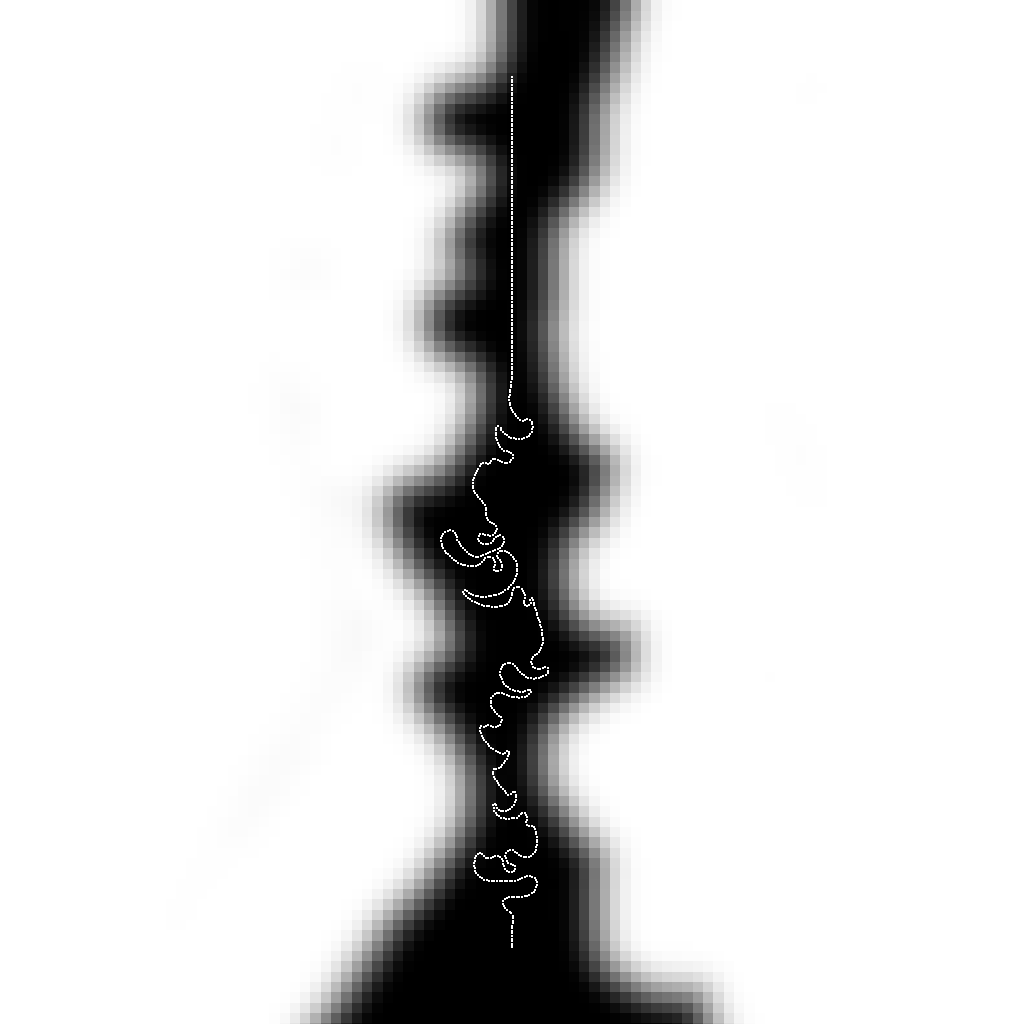
\includegraphics[width=\textwidth]{meander_terrain.png}
    \caption{Terreno com relevo ($1200$ passos).}
\end{subfigure}
\caption{Execução reproduzida da baseline em terreno plano e restrito por topografia.}
\label{fig:comparacao}
\end{figure}

\begin{figure}[t]
\centering
\begin{subfigure}[b]{0.48\columnwidth}
    \centering
    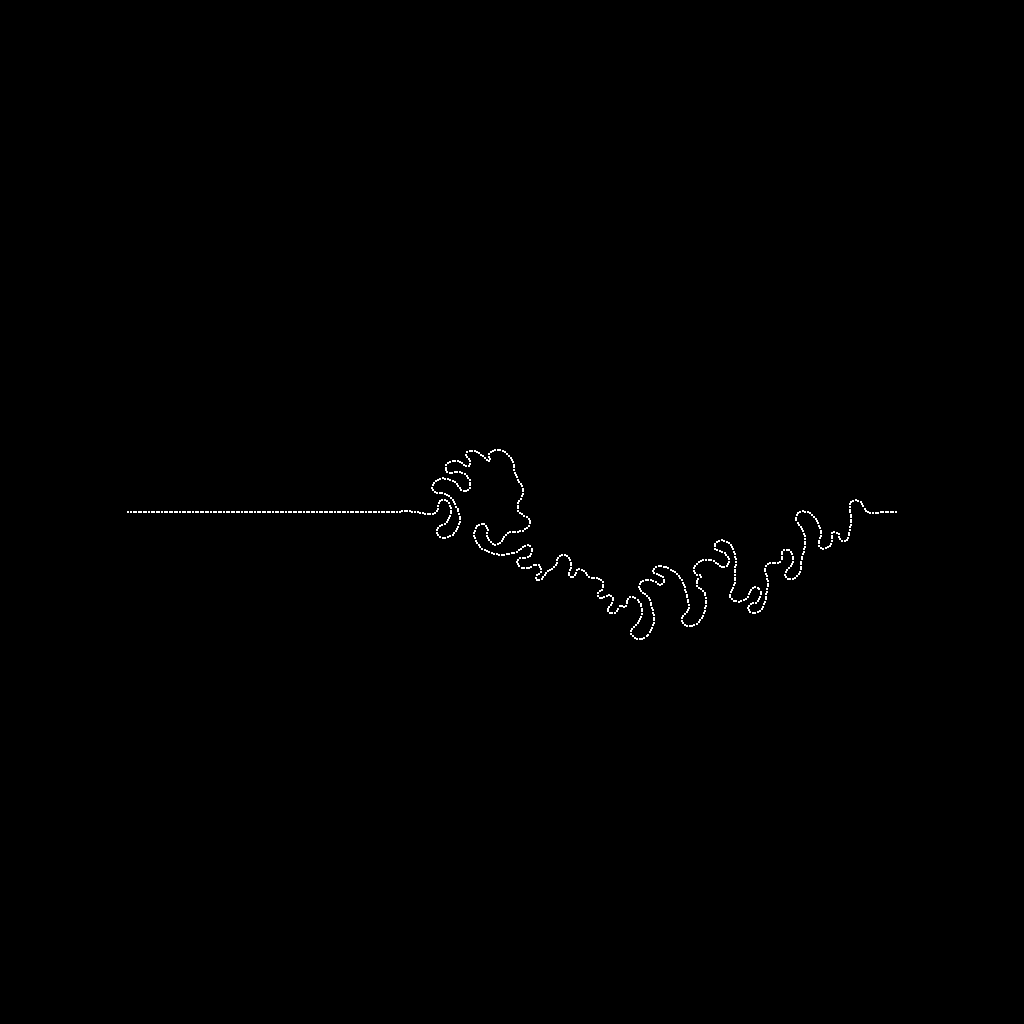
\includegraphics[width=\textwidth]{avulsion_before.png}
    \caption{Antes da avulsão (passo $700$).}
\end{subfigure}
\hfill
\begin{subfigure}[b]{0.48\columnwidth}
    \centering
    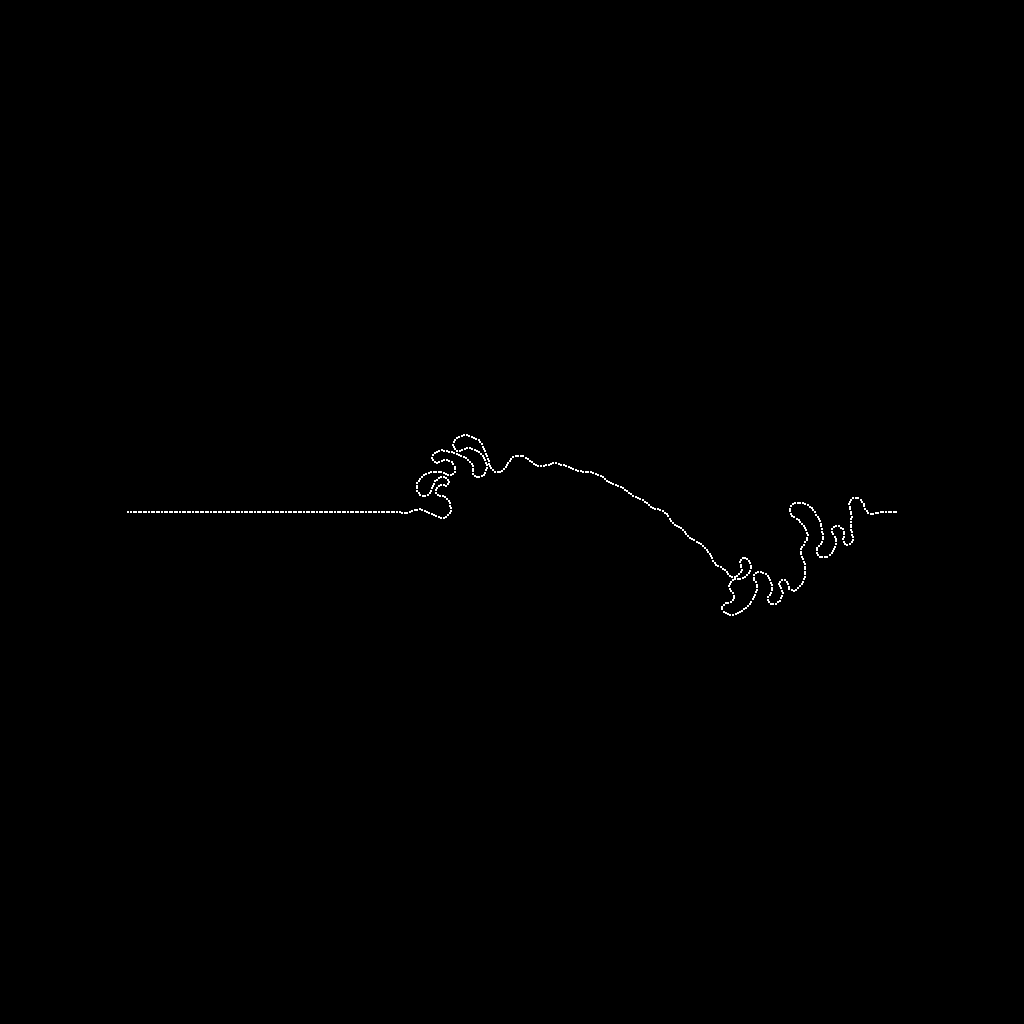
\includegraphics[width=\textwidth]{avulsion_after.png}
    \caption{Após avulsão ($+50$ passos).}
\end{subfigure}
\caption{Reprodução dos eventos topológicos de cutoff e avulsão da baseline.}
\label{fig:avulsion_check}
\end{figure}

% =============================================================================
\section{Discussão}
% =============================================================================
\orientacao{Interprete os resultados. Discuta ganhos, perdas, falhas, compromissos,
limitações, ameaças à validade e o que ainda precisaria ser testado antes de uma submissão.}

Os resultados preliminares do Checkpoint 2 confirmam que a formulação normalizada por $\bar{E}$ preserva estritamente o comportamento original quando o substrato é homogêneo ($L_\infty \le 10^{-9}$) e modifica de forma estável a trajetória quando há contraste litológico, sem introduzir instabilidades numéricas (\texttt{NaN}) durante a reamostragem por splines cúbicas.

Como próximos passos para a versão final do artigo, serão consolidadas as séries temporais completas de sinuosidade $S(t)$, contagem de \textit{cutoffs} com múltiplas sementes estocásticas, medição de tempo de execução via \texttt{std::chrono} e figuras comparativas sobrepondo o mapa litológico ao traçado do canal.

% =============================================================================
\section{Conclusão}
% =============================================================================
\orientacao{Retome o problema, sintetize a contribuição e os resultados mais importantes.
Não introduza novos experimentos. Indique trabalhos futuros concretos.}

Neste trabalho em andamento, apresentamos e implementamos uma extensão ao método de \textcite{paris2023meandering} para incorporar a mobilidade litológica relativa do substrato na simulação procedural de rios meândricos. A consulta na margem externa do canal demonstrou compatibilidade exata com a baseline em substratos uniformes e capacidade de modular localmente a migração lateral em substratos heterogêneos. Na etapa final do projeto, expandiremos a avaliação quantitativa e visual conforme o protocolo experimental estabelecido.

% =============================================================================
% REFERÊNCIAS
% =============================================================================
\balance
\printbibliography[title={Referências}]

\end{document}
